	% Szglab4
% ===========================================================================
%
\chapter{Analízis modell kidolgozása 2}

\thispagestyle{fancy}

\section{Objektum katalógus}

\subsection{Robot}

A robotok azok az eszközök, amelyek a játék során versenyeznek egymással. Minden robotra egy felhasználó jut, aki irányíthatja azt. A robotok tudnak elhelyezni a pályán a olajfoltokat és ragacsfoltokat is. A robotok ugrással tudnak a cellákon keresztül a pályán haladni. Minden robotnak van sebessége és természetesen egy aktuális pozíciója is. A robotok tudják magukról, hogy mekkora távolságot tettek már meg a játék során, valamit azt is, hogy még hány olaj- illetve ragacsfolttal rendelkeznek. A robotok egymással ütközhetnek, aminek bekövetkeztekor erről szintén értesülhetnek.

\subsection{Cella}

A cellák tudják magukról, hogy olajfoltosak-e, ragacsfoltosak-e, vagy éppen üresek-e, - azaz egyik folt sem található meg rajtuk. A cellák összessége eredményezi a versenyzésre kijelölt pályát. A cella felelőssége az, hogy ha rálép egy mozgó objektum, akkor annak el tudja végezni a megfelelő utasításait, ilyen például a sebesség megfelezése, folt elhelyezése önmagán, vagy a robotok megsemmisítése.

\subsection{Pálya}

A pálya a cellák összességéből tevődik össze, amiben üres cellák is lesznek, azaz lyukak. Ezen a pályán versenyeznek a robotok valójában. A pálya tisztában van azzal, hogy hol van cella, s hol nincs. (Azaz, hogy melyik koordinátára ugorva marad életben a robot és melyik koordinátára ugorva hal meg.) A pálya tudja megadni az adott koordinátájú cella szomszédos, üresen álló celláit is. Erre akkor van szükség, ha két robot egyszerre szeretne ugyanarra a cellára ugrani. A pálya további felelőssége még, hogy a robotokat egymással összeütköztesse, ha esetleg azonos cellára lépnének. 

\subsection{Olajfolt}

A olajfoltok cellákon helyezkedhetnek el, illetve robotok tudják őket elhelyezni továbblépésük előtt, s ezek módosító hatással vannak az ezt követően belelépő robotokra: a robot sebessége nem lesz módosítható, a következő ugrás sebességvektora így ugyanakkora lesz, mint az előzőé.

\subsection{Ragacsfolt}

A ragacsfoltok szintén a cellákon helyezkedhetnek el, illetve a robotok tudják őket elhelyezni a továbblépésük előtt, s ezek módosító hatással vannak az ezt követően belelépő robotokra: megfelezik a robotok sebességének a nagyságát, tehát lassító hatással bírnak.


\section{Statikus struktúra diagramok}
\comment{Az előző alfejezet osztályainak kapcsolatait és publikus metódusait bemutató osztálydiagram(ok). Tipikus hibalehetőségek: csillag-topológia, szigetek.}

\begin{figure}[h]
\begin{center}
%\includegraphics[width=17cm]{chapters/chapter04/example.pdf}
\caption{x}
\label{fig:example3}
\end{center}
\end{figure}


\section{Osztályok leírása}
\comment{Az előző alfejezetben tárgyalt objektumok felelősségének formalizálása attribútumokká, metódusokká. Csak publikus metódusok szerepelhetnek. Ebben az alfejezetben megjelennek az interfészek, az öröklés, az absztrakt osztályok. Segédosztályokra még mindig nincs szükség. Az osztályok ABC sorrendben kövessék egymást. Interfészek esetén az Interfészek, Attribútumok pontok kimaradnak.}

\subsection{Osztály1}
\begin{itemize}
\item Felelősség\\
\comment{Mi az osztály felelőssége. Kb 1 bekezdés.}
\item Ősosztályok\\
\comment{Mely osztályokból származik (öröklési hierarchia)\newline
Legősebb osztály $\rightarrow$ Ősosztály2 $\rightarrow$ Ősosztály3...}
\item Interfészek\\
\comment{Mely interfészeket valósítja meg.}
\item Attribútumok\\
\comment{Milyen attribútumai vannak}
	\begin{itemize}
		\item attribútum1: attribútum jellemzése: mire való
		\item attribútum2: attribútum jellemzése: mire való
	\end{itemize}
\item Metódusok\\
\comment{Milyen publikus metódusokkal rendelkezik. Metódusonként egy-három mondat arról, hogy a metódus mit csinál.}
	\begin{itemize}
		\item int foo(Osztály3 o1, Osztály4 o2): metódus leírása
		\item int bar(Osztály5 o1): metódus leírása
	\end{itemize}
\end{itemize}

\subsection{Osztály2}
\begin{itemize}
\item Felelősség\\
\comment{Mi az osztály felelőssége. Kb 1 bekezdés.}
\item Ősosztályok\\
\comment{Mely osztályokból származik (öröklési hierarchia)\newline
Legősebb osztály $\rightarrow$ Ősosztály2 $\rightarrow$ Ősosztály3...}
\item Interfészek\\
\comment{Mely interfészeket valósítja meg.}
\item Attribútumok\\
\comment{Milyen attribútumai vannak}
	\begin{itemize}
		\item attribútum1: attribútum jellemzése: mire való
		\item attribútum2: attribútum jellemzése: mire való
	\end{itemize}
\item Metódusok\\
\comment{Milyen publikus metódusokkal rendelkezik. Metódusonként egy-három mondat arról, hogy a metódus mit csinál.}
	\begin{itemize}
		\item int foo(Osztály3 o1, Osztály4 o2): metódus leírása
		\item int bar(Osztály5 o1): metódus leírása
	\end{itemize}
\end{itemize}

\section{Szekvencia diagramok}
\comment{Inicializálásra, use-case-ekre, belső működésre. Konzisztens kell legyen az előző alfejezettel. Minden metódus, ami ott szerepel, fel kell tűnjön valamelyik szekvenciában. Minden metódusnak, ami szekvenciában szerepel, szereplnie kell a valamelyik osztálydiagramon.}


\begin{figure}[!htbp]
	\begin{center}
		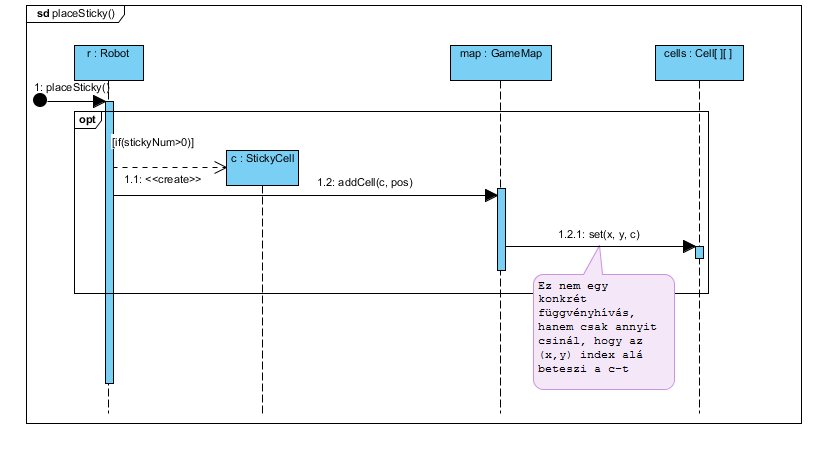
\includegraphics[width=166mm, center]{./chapters/chapter04/sticky.png}
		\caption{Ragacs hátrahagyása}
	\end{center}
\end{figure}

\begin{figure}[!htbp]
	\begin{center}
		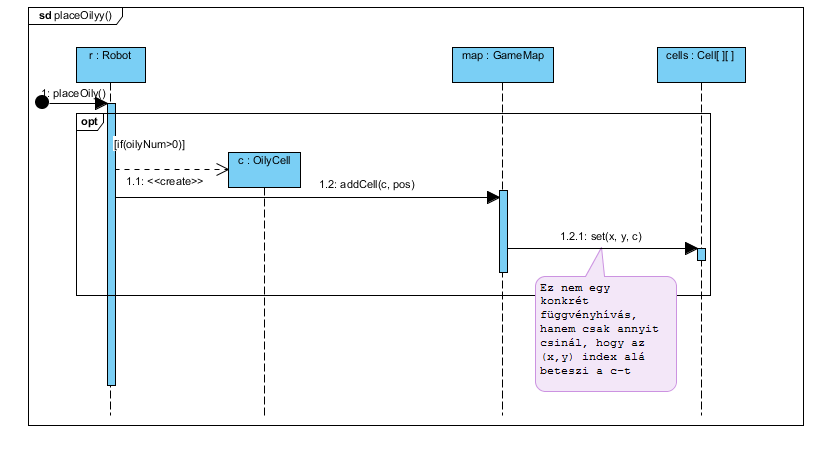
\includegraphics[width=166mm, center]{./chapters/chapter04/oily.png}
		\caption{Olaj hátrahagyása}
	\end{center}
\end{figure}

\clearpage

\begin{figure}[!htbp]
	\begin{center}
		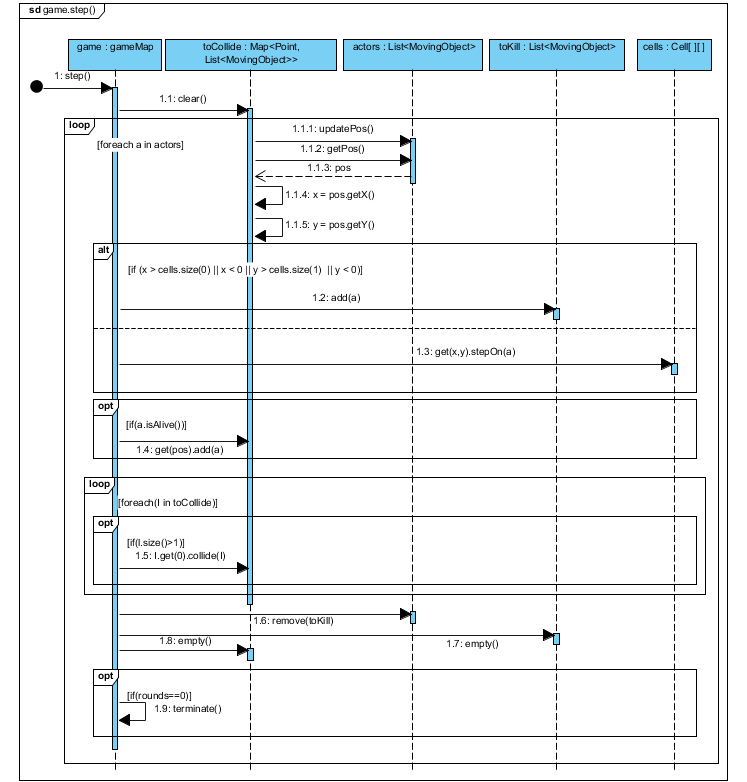
\includegraphics[width=195mm, center]{./chapters/chapter04/step.png}
		\caption{A játék léptetése}
	\end{center}
\end{figure}

\begin{figure}[!htbp]
	\begin{center}
		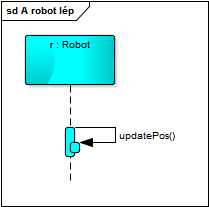
\includegraphics[width=100mm, center]{./chapters/chapter04/Arobotlep.png}
		\caption{}
	\end{center}
\end{figure}

\begin{figure}[!htbp]
	\begin{center}
		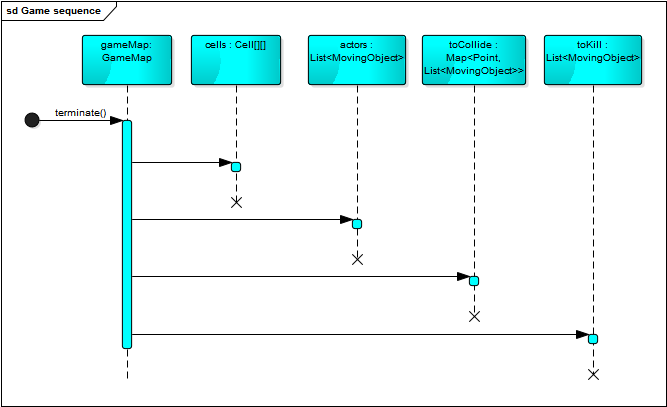
\includegraphics[width=180mm, center]{./chapters/chapter04/Gamesequence.png}
		\caption{}
	\end{center}
\end{figure}

\begin{figure}[!htbp]
	\begin{center}
		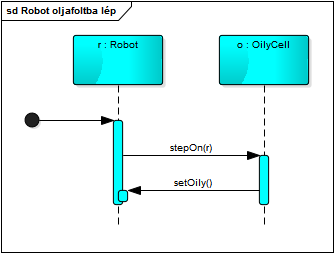
\includegraphics[width=100mm, center]{./chapters/chapter04/robotolajbalep.png}
		\caption{}
	\end{center}
\end{figure}

\begin{figure}[!htbp]
	\begin{center}
		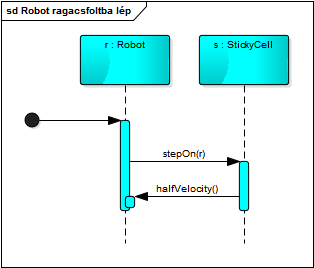
\includegraphics[width=100mm, center]{./chapters/chapter04/robotragacsbalep.png}
		\caption{}
	\end{center}
\end{figure}

\begin{figure}[!htbp]
	\begin{center}
		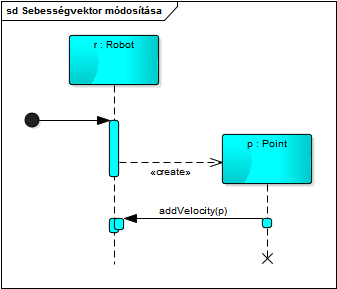
\includegraphics[width=100mm, center]{./chapters/chapter04/sebesseg.png}
		\caption{}
	\end{center}
\end{figure}

\section{State-chartok}
\comment{Csak azokhoz az osztályokhoz, ahol van értelme. Egyetlen állapotból álló state-chartok ne szerepeljenek. A játék működését bemutató state-chart-ot készíteni tilos.}

\begin{figure}[h]
\begin{center}
%\includegraphics[width=17cm]{chapters/chapter04/example.pdf}
\caption{x}
\label{fig:example3}
\end{center}
\end{figure}

